% mn2esample.tex
%
% v2.1 released 22nd May 2002 (G. Hutton)
%
% The mnsample.tex file has been amended to highlight
% the proper use of LaTeX2e code with the class file
% and using natbib cross-referencing. These changes
% do not reflect the original paper by A. V. Raveendran.
%
% Previous versions of this sample document were
% compatible with the LaTeX 2.09 style file mn.sty
% v1.2 released 5th September 1994 (M. Reed)
% v1.1 released 18th July 1994
% v1.0 released 28th January 1994

\documentclass[usenatbib]{mn2e}
\let\bibhang\relax
\usepackage{graphicx,subfigure}
\usepackage{bm}
\usepackage{longtable}
\usepackage{float}
\usepackage{amsmath,amssymb,graphicx}
\usepackage{rotating}
\usepackage{color}
\usepackage{cite}
\usepackage{epstopdf}

\bibliographystyle{mn2e}
\bibdata{sources}

% If your system does not have the AMS fonts version 2.0 installed, then
% remove the useAMS option.
%
% useAMS allows you to obtain upright Greek characters.
% e.g. \umu, \upi etc.  See the section on "Upright Greek characters" in
% this guide for further information.
%
% If you are using AMS 2.0 fonts, bold math letters/symbols are available
% at a larger range of sizes for NFSS release 1 and 2 (using \boldmath or
% preferably \bmath).
%
% The usenatbib command allows the use of Patrick Daly's natbib.sty for
% cross-referencing.
%
% If you wish to typeset the paper in Times font (if you do not have the
% PostScript Type 1 Computer Modern fonts you will need to do this to get
% smoother fonts in a PDF file) then uncomment the next line
% \usepackage{Times}

%%%%% AUTHORS - PLACE YOUR OWN MACROS HERE %%%%%

\newcommand{\f}[2]{\frac{#1}{#2}}

% denotes an edit in the actual body of the text.
%% denotes a personal comment by the editor.

%%%%%%%%%%%%%%%%%%%%%%%%%%%%%%%%%%%%%%%%%%%%%%%%


\title[]{High Altitude Ballooning: A Comprehensive Review}
\author[Amanda Maxham, etc.]{Amanda Maxham\thanks{E-mail:
maxham@physics.unlv.edu (AM); lujane@unlv.nevada.edu (EL); leeh44@unlv.nevada.edu (JL); maxham@physics.unlv.edu (IR) } Eric Lujan, Jake Lee, and Ian Rabago\\
Department of Physics and Astronomy, University of Nevada, Las Vegas, Las Vegas, NV, 89124, U.S.A.}
\begin{document}

\date{Accepted . Received ; }

\pagerange{\pageref{firstpage}--\pageref{lastpage}} \pubyear{2011}

\maketitle

\label{firstpage}
\begin{abstract}
This will be re-written after the paper is completed
\end{abstract}
\section{Introduction}
There has been a recent resurgance of interest in high altitude ballooning from universities, companies, hobbyists, scientists, and the general public. Since November of 2012, over 1,700 amateur balloon launches have been detected by APRS-IS \citep{arhab}. These launches have taken place on all continents (save for Antarctica) and have been orchestrated by hundreds of groups.

In this paper, the balloon's ascent and behaviour at altitude is described. Factors affecting balloon buoyancy with altitude are discussed in detail, namely membrane pressure, change in the gravitational constant $g$ with altitude, and air displacement caused by a solid payload. These factors, in combination, are thought to cause a balloon's free lift to decrease with altitude. One potential application of this natural lift change is the creation of a balloon that becomes neutrally buoyant at high-altitude without the use of a cutdown or other remote lift-altering device. Data from one of our launches is presented to illustrate an experimental example of a neutrally buoyant balloon and compare its observed behaviour with that which is theoretically described.

Finally, a thermodynamic model of high-altitude balloon motion is presented and analyzed.


%%The introduction should include the motive and purpose of the paper. The reader should be able to recognize the purpose of the entire paper by just reading this paragraph.

\section{Balloon Lift}

\subsection{Net Lift}

A free-floating balloon is acted upon by three forces along the z-axis. The upwards buoyant force, $F_B$, the gravitational force, $F_g$, and the drag force, $F_d$. These forces can be combined to find the net lift force of the balloon:

\begin{equation}
\Sigma F= F_B - F_g
\end{equation}

The buoyant force, $F_B$, can be calculated by using the Archimedes Equation:

\begin{equation}
F_{B} = \rho V
\end{equation}

where $\rho$ is the density of the displaced fluid in $kg/m^3$ (air, in the case of the balloon), V is the volume of the balloon in $m^3$, and g is the acceleration due to gravity in $m/s^2$. $F_{B}$ is in kilograms, as it is more convenient for our application.
The density and pressure of the atmosphere changes with altitude, causing the buoyant force to change throughout the flight. The data for density and pressure is available in the 1976 US Standard Atmosphere for up to 86 kilometers. The volume of the gas in the balloon can be measured with a flowmeter attached to the gas source.

The gravitational force, $F_g$, is the mass of the entire balloon, including the payloads, the balloon itself, and the gas inside the balloon:

\begin{equation}
F_{g}=m_b-m_p-(\f{n*M}{1000})
\end{equation}

where $m_b$ is the mass of the balloon, $m_p$ is the mass of the payload, $n$ is the moles of gas in the balloon, and $M$ is the mass of the gas in grams.

When both of these forces are combined into equation 1, we end up with the net lift, or $\Sigma F$. This value can be used for various calculations regarding the balloon. 

\subsection{Change In Lift With Altitude}
\label{sec:backpressure}

During several launches, it was observed that the latex balloon was able to reach neutral buoyancy without any manual changes to the balloon. This meant that the net lift of the balloon decreased with altitude, eventually reaching 0. Of the two forces involved in the net lift, only one can change throughout the flight: buoyancy.

Two factors are involved with buoyancy: The volume of the gas and the density of the air. The density of the air changes throughout the flight due to change in altitude. The volume of the gas also changes throughout the flight, and this can be modeled with the ideal gas law. 

\begin{equation}
Pv=nRt
\end{equation}

However, assuming that the pressure inside the balloon is the same as the pressure outside the balloon (the balloon expands to match the pressure), the volume of the balloon changes proportionally to the density of the atmosphere, resulting in no change in lift. This is contradictory to our observations; therefore, there has to be another factor that effects the volume. This is the back pressure of the elastic latex on the gas inside. 

Various models exist for sphere rubber shells (also known as rubber balloons), including the Gent model and the Mooney-Rivlin model. This paper will be focusing on the Mooney-Rivlin model too keep the paper concise.

The modified Mooney-Rivlin model for an incompressible spherical rubber shell is as such:

\begin{equation}
\Delta P = 2\mu\frac{t_0}{r_0}((\frac{t_0}{r_0})-(\frac{t_0}{r_0})^7)(1+\frac{1-\alpha}{\alpha}(\frac{t_0}{r_0})^2)
\end{equation}

Where $\mu$ is the shear modulus, $\alpha$ is a constant, $r_0$ is the unstretched radius of the balloon, $r$ is the inflated radius of the balloon, and $t_0$ is the thickness of the balloon. Setting $\alpha$ as 1 results in the neo-Hookean model. While this is useful for small stretches, it does not accurately describe experimental data at high values of strain "Kanner". The values in "Müller" suggest values of $\f{10}{11}$ for $\alpha$ and $300 kPa$ for $\mu$.

\subsection{Neutral Buoyancy}

Achieving neutral buoyancy is the foundation of achieving long-distance balloon flight. When a balloon is neutrally buoyant, it is able maintain suspension in the atmosphere and thus be exposed to high-altitude wind currents for a larger duration. Most trans-continental and trans-oceanic flights attain near-neutral buoyancy and maintain it for long periods of time, allowing them to travel long distances for extended periods of time.

Neutral buoyancy is achieved when the forces on the balloon along the z-axis reach a point of equalibrium so that:

\begin{equation}
	F = 0 = F_B - F_g
\end{equation}

Which can be manipulated to show equivalence between buoyant force and gravity:

\begin{equation}
	F_B = F_g
\end{equation}

In practice, this is acheived by filling the balloon with an excess of gas that creates a small net initial upwards force (in excess of gravity) that diminishes over the course of the flight (see Section~\ref{sec:backpressure}).

Initial net upwards lift is critical to the balloon's buoyancy at a target altitude. Adding too much gas at the launch point will cause the balloon to burst before it can become neutrally buoyant. A shortage of initial gas will cause the force of gravity to exceed the buoyant force at the target altitude and cause the balloon to sink.

There is no "magic amount" of extra lift that guarantees neutral buoyancy. The amount of extra lift required is dependent on the size of the balloon, atmospheric conditions, the type of lift gas used, and the mass of the payload.

Our team launched a neutrally-buoyant balloon from Mesquite, Arizona, USA, on August 4, 2013 at 16:29 UTC.
Its ascent path is plotted below:

\begin{figure}[!ht]
  \begin{center}
  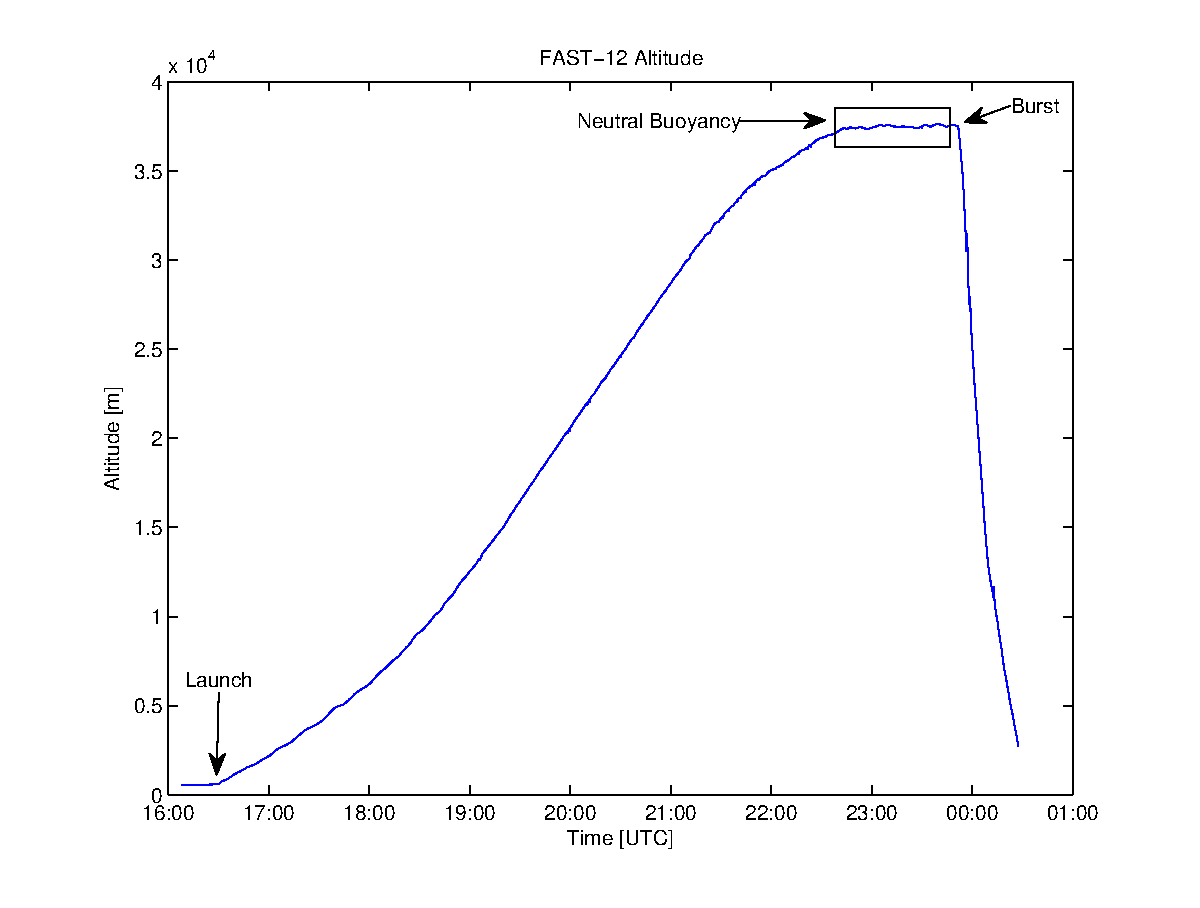
\includegraphics[width=0.5\textwidth]{altitude.eps}
  \caption{Altitude of neutrally-buoyant balloon vs. time}
\end{center}
\end{figure}



\section{Burst Altitude}

\subsection{Balloon Elasticity}

\section{The effect of wind vectors on the ascent and descent paths of high-altitude balloons}

\subsection{Experimental Examples}

\label{lastpage}
\bibliography{sources}
\end{document}
